\documentclass{acm_proc_article-sp}

\usepackage{graphicx}
\usepackage{amsmath}
\usepackage{float}
\usepackage{natbib}
\usepackage{url}
\usepackage{amssymb}

%\usepackage{fancyhdr}
%\lfoot{HELLO}\cfoot{\thepage}\rfoot{WORLD}

\begin{document}
\title{Analysis of an Adaption of the Adaptive Aggressive Algorithm: Asking are AA Algorithms Actually All that Accurate in Applicable Auctions Anyway?}
\numberofauthors{3} 
\author{
  \alignauthor
    Rupert Bedford\\
    \email{rb9281@bristol.ac.uk}
  \alignauthor
    Max Robinson\\
    \email{mr9388@bristol.ac.uk}
  \alignauthor
    Jonathan Simmonds
    \email{js9721@bristol.ac.uk}
}
\date{7 December 2012}

\maketitle
\begin{abstract} \label{sec:abstract}
\begin{verbatim}
                             .::::. 
                           .::::::::. 
                           ::::::::::: 
                           ':::::::::::.. 
                            :::::::::::::::' 
                             ':::::::::::. 
                               .::::::::::::::' 
                             .:::::::::::... 
                            ::::::::::::::'' 
                .:::.       '::::::::'':::: 
              .::::::::.      ':::::'  ':::: 
             .::::':::::::.    :::::    '::::. 
           .:::::' ':::::::::. :::::      ':::. 
         .:::::'     ':::::::::.:::::       '::. 
       .::::''         '::::::::::::::       '::. 
      .::''              '::::::::::::         :::... 
   ..::::                  ':::::::::'        .:' '''' 
..''''':'                    ':::::.' 
\end{verbatim}
\end{abstract}

\pagebreak

\section{Introduction} \label{sec:introduction}
% OWNER: Rupert
% - What is automated trading (history)
% - What our goal was

An automated trader is an algorithm that automatically places trading orders on
an electronic market.
The trader receives buy or sell orders from customers with a price and
quantity.
The trader makes money by buying for less than the customers price or selling
for more than the customers price.
Therefore the goal of a trading strategy is maximise these margins and the
trading volume to maximise the amount of profit.

In a double auction buyers submit bids to the market and sellers submit asks.
When a bid equals or exceeds a seller's asks the bid is accepted and the trade
occurs. Experiments have shown (Smith 1962) that the prices in the market will
rapidly converge on the price equilibrium in a number of market environments.

IBM published a paper in 2001 that showed that their MGD trading strategy and
Dave Cliff's ZIP were able to outperform human traders.
Algorithmic strategies are able to react more quickly to changing market
conditions and combine information from a multiple sources.

In this paper we experiment with different trading strategies for the
continuous double auction.
We have implemented the Adaptive Aggressiveness trading algorithm and compared
its performance with other adaptive algorithms as well as simpler traders.\\


\section{Environment} \label{sec:environment}
\subsection{BSE} \label{sec:BSE}
For this assignment we use the Bristol Stock Exchange (BSE) as a virtual trading environment or, 
more accurately, a minimal simulation of a limit order book financial exchange. As it is 
minimalistic it has the advantage of being both easy to understand and quick to run.

BSE acts like a dark pool continuous double auction as both buyers and sellers simultaneously bid 
towards their limit price and can see all other offers but do not know the identity of the trader.
Only a single commodity is traded. 
This has a number of implications, the main one being the difficulty of implementing the MGD trader 
in this environment as it requires non-anonymised data to calculate which trades have been updated 
each time step. This is covered in more detail in Section \ref{sec:traders_GDV}. Other traders (e.g. 
ZIP and AA) do not have this limitation.\\


\subsection{Traders} \label{sec:traders}
\subsubsection{ZIP} \label{sec:traders_ZIP}
% OWNER: Jonny
% - What was significant --- key points
% - Advantages/disadvantages
Zero-Intelligence-Plus (ZIP) traders.\\


\subsubsection{GD Variants} \label{sec:traders_GDV}
% OWNER: Rupert
% - Shavers / Sniper / XKCD, etc.
% - MGD anonymised data (see BSE paragraph 2)
% - We implemented it but couldn't do a full implementation

The Gjerstad Dickhaut (GD) trading strategy was invented by John Dickhaut and
Steven Gjerstad in their 1998 paper \emph{Price Formation in Double
Auctions}\cite{gd}.
GD works by building a belief function of whether a bid at a particular price
will be accepted by a seller.
The buyer then aims to maximise their profit through a combination of margin
and chance of trading.
The belief values are formed based on observed trades and outstanding shouts.
The GD strategy makes some simple assumptions such as if a bid was rejected a
lower bid will also be rejected since it will be less attractive to a seller.
The results of the experiments showed that GD has a higher efficiency than ZI.
The efficiency is the margin divided by the maximum theoretically margin
(difference between limit and price equilibrium).
They also showed that GD was able to cope with changing supply and demand
conditions.

Modified Gjerstad Dickhaut (MGD) \cite{mgd} is a version of GD that
is better suited to volatile conditions that can occur at the start of a
session where there is very little information about accepted and rejected
orders.
An MGD agent remembers the highest and lowest prices from the last session.
A MGD buyer will then set the belief function to 1 for all prices above the
lowest price and to 0 for all prices below the lowest price.
MGD is also able to hold multiple units.

GDX\cite{gdx} is a Dynamic Programming based variant of GD.
GDX uses the same belief function as GD but uses Dynamic Programming to
maximise the long term reward instead of the short term reward.
Dynamic Programming is used to compute optimal policies in Markov Decision
Problems.
The emphasis placed between short and long term rewards can be controlled using
the discount value ($\gamma$).
$\gamma = 0$ will result in the same behaviour as the standard GD strategy
(short-term reward) while $\gamma = 1$ will cause GDX to maximise the long term
reward.
However setting $\gamma$ close to 1 will cause GDX to always wait for a better
deal and thus not make any trades.
They found that under certain market environments GDX was able to outperform
both GD and ZIP.
With a $\gamma$ between 0.75 and 0.85 GDX always outperforms GD.
GDX is more flexible than GD and can handle multiple goods although
optimisations are needed to keep the state space tractable.

The Zero Intelligence (ZIC) trader does not learn from market events (Gode
1993).\\


\pagebreak % QUESTIONABLE
\subsection{Adaptive Aggressive Traders} \label{sec:AA}
% OWNER: Max
% - ???

The adaptive aggressive algorithm relies on the principal that you can be in
two different states. One where you trade more frequently closer to your limit
price, higher chance of trading but lower profit per trade. The other where you
trade further from your limit price, which decreases the likelihood of making a
trade but increases the amount of profit you will make when you do trade.

The Adaptive-Aggressive algorithm maintains an aggressiveness value (r), which
determines how close to your limit price you will be trading. A completely
aggressive buyer ($r = 1$) will buy at their limit price, and a completely
passive trader ($r = -1$) will buy at the minimum market price (\$1 in our case)
\subsection{Price Equilibrium Estimator}
One of the key features that most trading algorithms rely on is the ability to
estimate the equilibrium price of the market. For this we used the following
equation which estimates the market equilibrium price based on the N most
recent transactions, known as a moving average.

\begin{equation}
\hat p^* = \frac{\sum^T_{i=T-N+1}w_ip_i}{\sum^T_{i=T-N+1}w_i}\\
\text{where $w_T = 1$ and $w_{i-1} = \lambda w_i$}
\label{equest}
\end{equation}

The $w_i$ represents the weight of the transaction so that we weight more
recent transactions more heavily with the $\lambda$ affect how severe this
weighting is. We set the value of $\lambda$ to 0.9 which was the value
recommended in the original paper \cite[p.~100]{AA_thesis}.\\

We also tested $\lambda$ values from $0$ to $1$ in $0.1$ increments over 8000 
market sessions (of 600 timesteps each) to find their effect on AA's performance. We didn't find any
statistically significant difference between the different values. Our results
are included in table \ref{tbl:lambda_results}.
\begin{table}
  \centering
  \label{tbl:lambda_results}
  \begin{tabular}{ | c | c | }
    \hline
    \textbf{$\lambda$ value} & \textbf{Average finishing balance (3dp)} \\
    \hline
    0.0 & 128.048 \\
    0.1 & 128.040 \\
    0.2 & 128.041 \\
    0.3 & 128.314 \\
    0.4 & 128.268 \\
    0.5 & 128.278 \\
    0.6 & 128.224 \\
    0.7 & 128.380 \\
    0.8 & 128.172 \\
    0.9 & 128.365 \\
    1.0 & 128.462 \\
    \hline \hline
    ZIC & 89.521 \\
    ZIP & 116.719 \\
    \hline
  \end{tabular}
\end{table}

\subsubsection{Price estimation} \label{sec:AA_price_estimation}
% OWNER: Max
% - Graph of all trades with projected price equilibrium
% - MEGA GRAPH

\begin{figure}
  \centering
  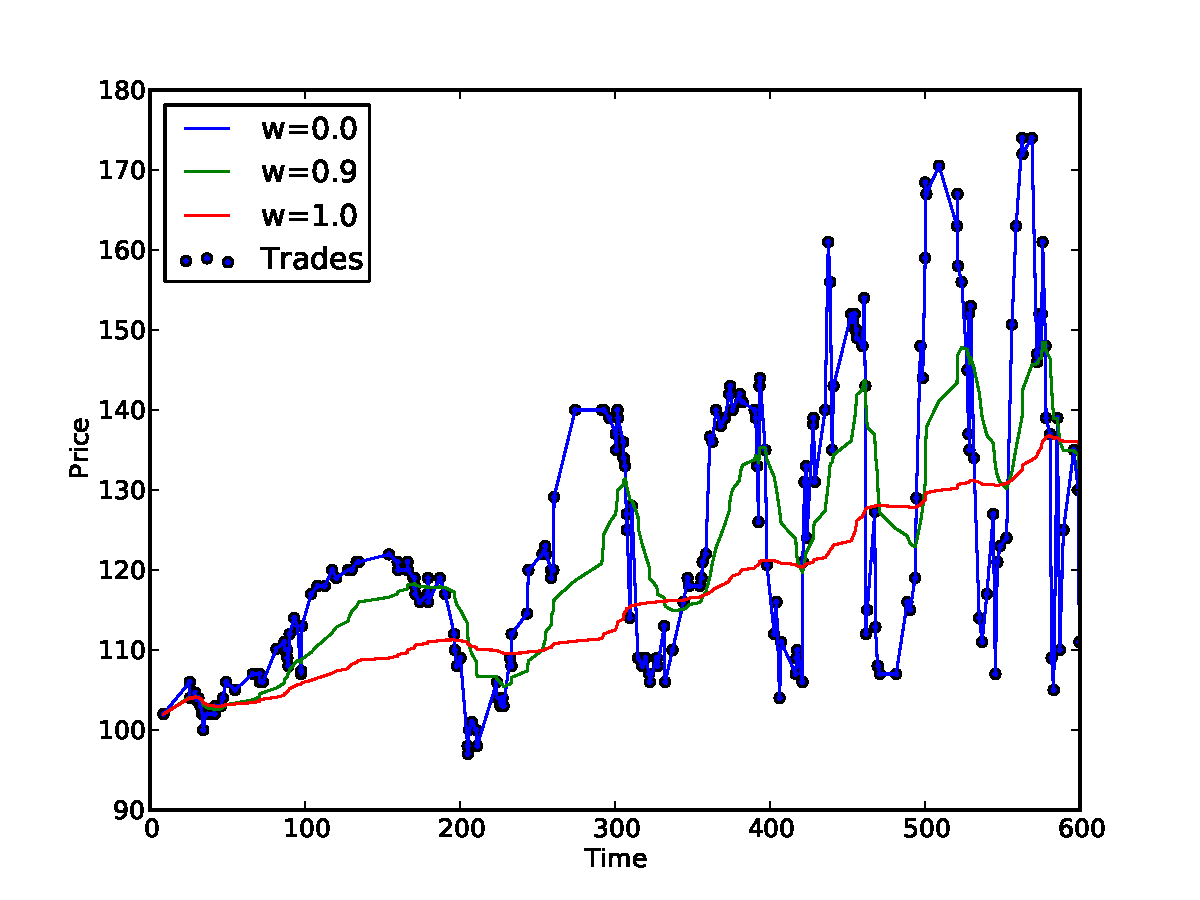
\includegraphics[width=\columnwidth]{graphs_and_stats/equilibriums.pdf}
  \caption{The affect of the weighting value on the price equilibrium
  estimate.}
\end{figure}

Short term learning reflects how the value of our aggressive is calculated and
then subsequently updated. However, first we must define two concepts. An
intra-marginal trader is a trader that bids above the equilibrium if they are a
buyer (or asks below the equilibrium if they are a seller). Whereas an
extra-marginal trader will never trade above the equilibrium if they are a
buyer (or below the equilibrium if they are a seller).

Whether our trader is acting in an extra-marginal or intra-marginal capacity
will depend upon the limit price for our order. If we have a limit price above
the equilibrium (below the equilibrium for a seller) then we are considered an
intra-marginal trader otherwise we are considered extra-marginal.

The price that we then submit will depend upon which capacity we are acting
under based on the follow equations.

\textbf{Intra-marginal buyer}
\begin{equation}
\tau =
\begin{cases}
      \hat{p}^*(1- \frac{e^{-r\theta}-1}{e^{\theta}-1}), &  \text{if r } \in (-1,0)  \\
      \hat{p}^* + (l_i-\hat{p}^*)(\frac{e^{r\theta}-1}{e^\theta-1}), & \text{if
      r } \in (0,1)
\end{cases}
\label{intrabuyer}
\end{equation}

where $\theta$ (\ref{sec:AA_long_term_learning}) measures the volatility of the
market, $l_i$ is the limit price for the buyer, $\hat{p}^*$ is the estimator of the
equilibrium price.

\textbf{Extra-marginal buyer}
\begin{equation}
\tau =
\begin{cases}
      l_i(1-\frac{e^{-r\theta}-1}{e^\theta-1} &  \text{if r } \in (-1,0)  \\
      l_i & \text{if r } \in (0,1)
\end{cases}
\label{extrabuyer}
\end{equation}

\textbf{Intra-marginal seller}
\begin{equation}
\label{intraseller}
\tau =
\begin{cases}
      \hat{p}^* + (MAX-\hat{p}^*)( \frac{e^{-r\theta}-1}{e^{\theta}-1}), &  \text{if r } \in (-1,0)  \\
      c_j + (\hat{p}^*-c_j)(1-\frac{e^{r\theta}-1}{e^\theta-1}), & \text{if r } \in (0,1)
\end{cases}
\end{equation}

where MAX is the maximum value that can be submitted to the market and $c_j$ is
the limit price for the seller.

\textbf{Extra-marginal seller}
\begin{equation}
\tau =
\begin{cases}
      c_j + (MAX-c_j)(1-\frac{e^{-r\theta}-1}{e^\theta-1} &  \text{if r } \in (-1,0)  \\
      c_j & \text{if r } \in (0,1)
\end{cases}
\label{extraseller}
\end{equation}

In the paper, there was a different value used instead of $\theta$, designed to
ensure that the curve provided by the equations was continuous. However, we
found that just using $\theta$ was still sufficiently accurate and greatly
simplified the above equations.

One of the equations is then used to determine the ideal price that we want to
be trading at. We then use the following rules to determine the actual shout
that we will make when asked to submit a new order. The $o_{bid}$ and $o_{ask}$
represent the best bid (highest) and best ask (lowest) on the market that have
not yet been accepted. The value of $\eta$ is set as a parameter and reflects
how quickly we converge on our estimated price (higher $\eta$ converge slower).

\textbf{Bidding rules for Buyer}
if ($l_i \leq o_bid$) - Submit no bid (market transacting above our limit)\\
else submit bid given by Equation \ref{bidieqn}

\begin{equation}
bid_i = \frac{o_{bid} + (\tau - o_{bid}}{\eta}
\label{bidieqn}
\end{equation}

\textbf{Bidding rules for Seller}
if ($c_j \geq o_{ask}$) - Submit no ask (market transacting below our limit)\\
else submit bid given by Equation \ref{askieqn}

\begin{equation}
ask_i = o_{ask} - \frac{o_{ask}-\tau}{\eta}
\label{askieqn}
\end{equation}

Since these all require an existing bid on the market, there were difficult
rules that were used to determine what shout to make if we were the first
trader selected to make a bid. These can be found in the Adaptive Aggressive
paper \cite[p.~32]{AA_paper} but are not defined here.

Initially when we ran our algorithm we found that it was occasionally making a
loss upon receiving a new order from the scheduler with a different limit
price. The reason for this was that our previous bids had been submitted using
the limit price from the previous order. Since on the Bristol Stock Exchange it
is not possible to remove a bid, we added additional logic to notify us of the
new order. If it was found that the new order contained a limit that was
outside of our trading range, we cleared our previous bid using a stub.\\


\subsubsection{Short term learning} \label{sec:AA_short_term_learning}
% OWNER: Max
% - Graphs - r vs price equilibrium.
The aggressiveness of the Adaptive Aggressive algorithm is updated at every
time step using Equation \ref{updateaggressive} based on the following rules.

\textbf{Learning Rules for Buyer:}
if (trade occurs at price q)\\
    \indent if ($\tau \geq q$) be less aggressive (our price too high)\\
    \indent else be more aggressive ( our price too low)\\
else if ($\tau \leq o_bid$) be more aggressive ( our price too low)

\textbf{Learning Rules for Seller:}
if (trade occurs at price q)\\
    \indent if ($\tau \leq q$) be less aggressive (our price too low)\\
    \indent else be more aggressive ( our price too high\\
else if ($\tau \leq o_bid$) be more aggressive ( our price too high)

\begin{equation}
r(t+1) = r(t) + \beta_1(\delta(t) - r(t))\\\delta(t) = (1 \pm
\lambda_r)r_{shout} \pm \lambda_a
\label{updateaggressive}
\end{equation}

$\lambda_r$ and $\lambda_a$ representive the relative and absolute change in
r respectively. The absolute change exists to prevent r from never being able
to escape from a value of 0. Depending on the rules above, we either set the
two values to positive to become more aggressive or negative to become less
aggressive.\\

The aggressive is depending on our limit price and the current market state as
is illustrated in Fig. \ref{aavtime}. In order to collect more data, we
increases the scheduler to distribute items every five timesteps instead of
every thirty. This increases the number of trades in the market which in turn
provides us with a far more accurate estimate of the price equilibrium and more
trading data to work with.

One of the first conclusions we can draw from the graph is that our trader is
always playing an active role in the market, that is they are trading above the
market equilibrium. The reason for this is that the scheduler was set to
periodic meaning that the limit prices were provided in order to create the
sine wave visibile in Fig. \ref{aavtime}. Therefore, everyone receives limit
prices close to each other meaning that we have a competitive market which
means we have to trade close to our limit price. This is further reinforced by
the short order duration making it difficult to wait for a trade.

Initially our trader has a lower aggressiveness value (close to zero), this is
because the trader lacks information about the market and therefore adopts a
more passive role to prevent selling far above the equilibrium

The dips in the aggressiveness correspond to the falling equilibrium price
where we can afford to trade further below our limit price. 
\begin{figure} 
  \centering
  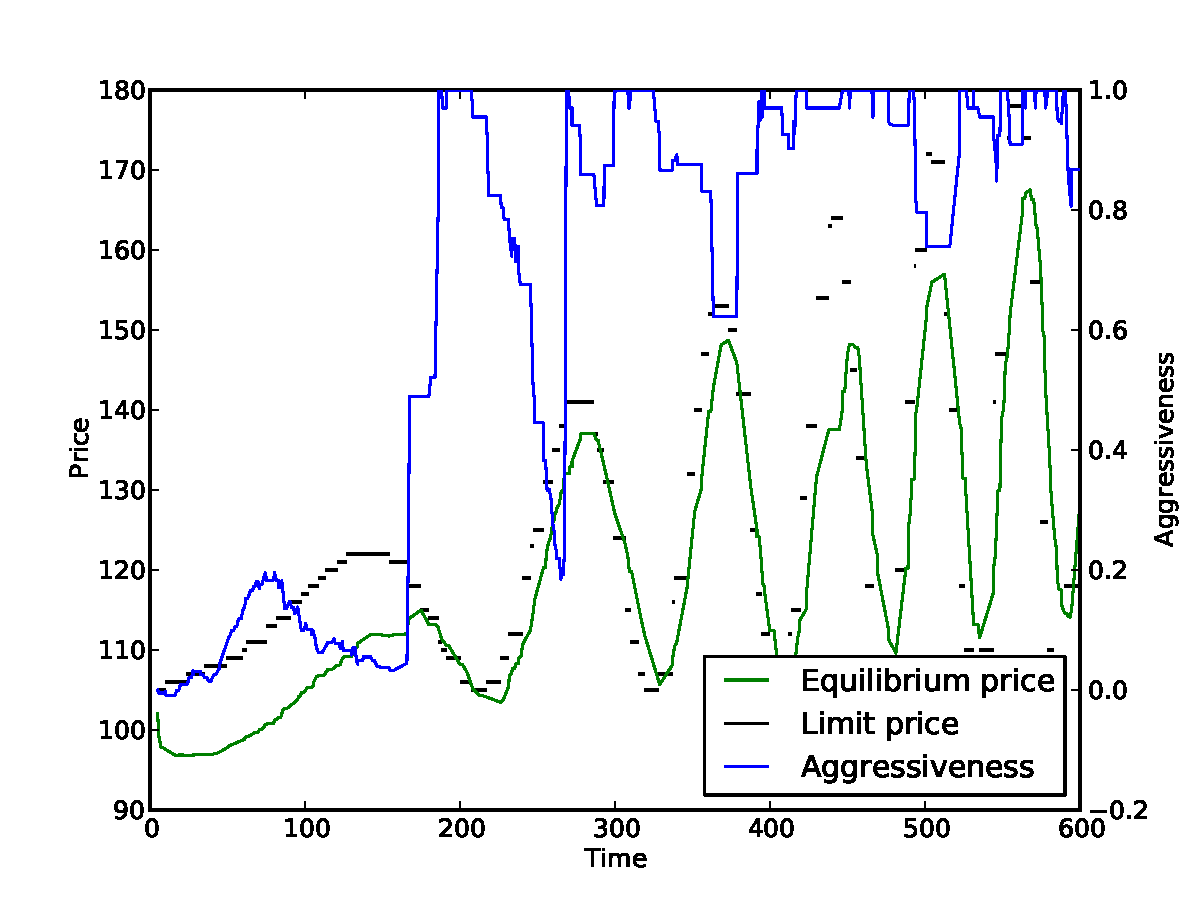
\includegraphics[width=\columnwidth]{graphs_and_stats/aggressiveness_vs_price.pdf}
  \label{aavtime}
  \caption{Aggressive and Price equilibrium throughout a trading day}
\end{figure}

\subsubsection{Long term learning} \label{sec:AA_long_term_learning}
% OWNER: Max
% - theta
Text.\\


\section{Calibration} \label{sec:calibration}
% OWNER: Group
% - $\beta_1$, $\beta_2$, $\gamma$, $\eta$
% - potential to compare statistically?
Text.\\


\section{Results} \label{sec:results}
% OWNER: Group
% - Graph: Average balance over time
% - Statistical analysis - why you used a certain test
%   Ed's report: ``According to the conducted Wilcoxon-Mann-Whitney two-tailed rank-sum tests, the difference in the observed efficiencies is significant ($U = 2, N_1 = N_2 = 10, p < 0.0003$)."
% - Experiment with changing scheduler
% - Other graphs

\begin{table}
  \centering
  \begin{tabular}{ | c | c | }
    \hline
    Strategy & Average Balance \\
    \hline
    ZIC & $93.863$ \\
    \hline
    SHVR & 106.139 \\
    \hline
    ZIP & 120.434 \\
    \hline
    AA & 136.555 \\
    \hline
  \end{tabular}
  \caption{Average balances for different trading strategies.}
\end{table}


\section{Conclusion} \label{sec:conclusion}
% OWNER: Group
% - Thank you and good night
% - Hold for applause
Text.\\


%\pagebreak
\bibliographystyle{unsrt}
\bibliography{algo_report}
\end{document}
